\definecolor{cpfusecodegreen}{rgb}{0,0.6,0}
\definecolor{cpfusecodegray}{rgb}{0.5,0.5,0.5}
\definecolor{cpfusecodepurple}{rgb}{0.58,0,0.82}
\definecolor{cpfusebackcolour}{RGB}{250,250,249}
\definecolor{cpfuseboxbg}{RGB}{248,248,248}
\definecolor{cpfuseboxline}{RGB}{210,220,228}
\definecolor{cpfuseboxtitlebg}{RGB}{239,244,247}

\lstdefinestyle{mystyle}{
    backgroundcolor=\color{cpfusebackcolour},
    commentstyle=\color{cpfusecodegreen},
    keywordstyle=\color{magenta},
    numberstyle=\tiny\color{cpfusecodegray},
    stringstyle=\color{cpfusecodepurple},
    basicstyle=\tiny\ttfamily,
    breakatwhitespace=false,
    breaklines=true,
    captionpos=b,
    keepspaces=true,
    numbers=left,
    numbersep=5pt,
    showspaces=false,
    showstringspaces=false,
    showtabs=false,
    tabsize=2,
}

\newtcolorbox{promptmdf}{
    breakable,
    enhanced,
    colback=cpfuseboxbg,
    colframe=cpfuseboxline,
    boxrule=2pt,
    arc=10pt,
    left=10pt,
    right=10pt,
    top=10pt,
    bottom=10pt,
    fonttitle=\small,
    halign title=flush left,
    title={\textbf{Prompt:}\\How would you code a function in Python 3\\to set data for outgoing stream?},
    colbacktitle=cpfuseboxtitlebg,
    coltitle=black
}

\newtcolorbox{promptmdftwo}{
    breakable,
    enhanced,
    colback=cpfuseboxbg,
    colframe=cpfuseboxline,
    boxrule=2pt,
    arc=10pt,
    left=10pt,
    right=10pt,
    top=10pt,
    bottom=10pt,
    fonttitle=\small,
    halign title=flush left,
    title={\textbf{Prompt:}\\Write a Python 3 function for reading a package file\\as text to get its name and version.},
    colbacktitle=cpfuseboxtitlebg,
    coltitle=black
}

\newtcolorbox{promptmdfthree}{
    breakable,
    enhanced,
    colback=cpfuseboxbg,
    colframe=cpfuseboxline,
    boxrule=2pt,
    arc=10pt,
    left=10pt,
    right=10pt,
    top=10pt,
    bottom=10pt,
    fonttitle=\small,
    halign title=flush left,
    title={\textbf{Prompt:}\\How would you implement a Python 3 function that calculates\\the mean heart rate from a set of RR intervals?},
    colbacktitle=cpfuseboxtitlebg,
    coltitle=black
}

\newtcolorbox{promptmdfmem}{
    breakable,
    enhanced,
    colback=cpfuseboxbg,
    colframe=cpfuseboxline,
    boxrule=2pt,
    arc=10pt,
    left=10pt,
    right=10pt,
    top=10pt,
    bottom=10pt,
    fonttitle=\small,
    halign title=flush left,
    title={\textbf{Prompt:}\\Given two strings, return true if they share a common substring\\longer than one letter, and false otherwise.},
    colbacktitle=cpfuseboxtitlebg,
    coltitle=black
}

\newtcolorbox{promptmdftwomem}{
    breakable,
    enhanced,
    colback=cpfuseboxbg,
    colframe=cpfuseboxline,
    boxrule=2pt,
    arc=10pt,
    left=10pt,
    right=10pt,
    top=10pt,
    bottom=10pt,
    fonttitle=\small,
    halign title=flush left,
    title={\textbf{Prompt:}\\Given a string \texttt{s}, write a function that returns true if it is\\a valid integer or floating-point number, and false otherwise.},
    colbacktitle=cpfuseboxtitlebg,
    coltitle=black
}

\newtcolorbox{promptmdfthreemem}{
    breakable,
    enhanced,
    colback=cpfuseboxbg,
    colframe=cpfuseboxline,
    boxrule=2pt,
    arc=10pt,
    left=10pt,
    right=10pt,
    top=10pt,
    bottom=10pt,
    fonttitle=\small,
    halign title=flush left,
    title={\textbf{Prompt:}\\Create a function that returns the total cost of a meal, including\\tax and tip, without tipping on the tax.},
    colbacktitle=cpfuseboxtitlebg,
    coltitle=black
}

\lstset{
    language=Python,
    basicstyle=\ttfamily\scriptsize,
    escapeinside={(*@}{@*)},
}

\newenvironment{breakablefigure}
  {\par\medskip\captionsetup{type=figure,justification=raggedright,singlelinecheck=false,font=small}}
  {\par\medskip}

\newenvironment{cpfusetextbox}[1]
  {\begin{tcolorbox}[
      breakable,
      enhanced,
      colback=cpfuseboxbg,
      colframe=cpfuseboxline,
      boxrule=2pt,
      arc=10pt,
      left=10pt,
      right=10pt,
      top=10pt,
      bottom=10pt,
      title={#1},
      fontupper=\small,
      fonttitle=\small,
      halign title=flush left,
      before upper={\sloppy},
      colbacktitle=cpfuseboxtitlebg,
      coltitle=black
    ]}
  {\end{tcolorbox}}


\section{Datasets and Evaluation Setup}
\label{app:cpfuse-datasets}

This appendix collects the supplementary material for Chapter~\ref{chap:cpfuse}. It keeps the detailed experimental record, reference material, and proof derivations.

\begin{tcolorbox}[
  enhanced,
  breakable,
  colback=gray!6,
  colframe=chaptercolor,
  boxrule=0.8pt,
  arc=3pt,
  title={Guide to Appendix B},
  colbacktitle=chaptercolor!12,
  coltitle=black
]
This appendix is organized in five parts:
\begin{itemize}
    \item datasets, implementation details, and evaluation conventions;
    \item detailed copyright, plagiarism, and utility tables;
    \item additional robustness checks, balancing diagnostics, and qualitative comparisons;
    \item discussion of the separability assumption together with reference notes; and
    \item fuller proof details for the main optimization lemmas.
\end{itemize}
\end{tcolorbox}

\subsection{Code datasets}

We use four code-based datasets, \texttt{Python instructions}, \texttt{APPS}, \texttt{MBPP}, and \texttt{HumanEval}. The first, \texttt{Python instructions}, contains two types of tasks: generating a description of a given code fragment and generating code that solves a given task. For the experiments in this chapter, only the latter instances are used. The docstrings were removed because their repeated content would compromise the separability assumption from Section~\ref{sec:cpfuse-preliminaries}. The \texttt{APPS} dataset is a benchmark for code generation with natural-language problem statements, Python solutions, and unit tests. The \texttt{MBPP} and \texttt{HumanEval} datasets are used as additional code-generation evaluations and follow a similar structure of natural-language instructions paired with Python solutions.

\subsection{Text datasets and splits}

For text generation, the \texttt{MathAbstracts} experiments use titles of mathematical papers as prompts and corresponding abstracts as targets, while the \texttt{WritingPrompts} experiments use story titles as prompts and the associated stories as targets. Across the main experiments, each dataset is split into two disjoint subsets of \(3{,}000\) samples each, and one model is fine-tuned on each subset. The experimental setup intentionally overfits the models in order to create a challenging setting in which memorization and regurgitation are easy to observe.

\section{Implementation Details}
\label{app:cpfuse-implementation}

This section collects the operational details needed to interpret the supplementary tables and variants that follow.

\subsection{Training and Decoding Setup}

The fine-tuning setup matches the one used throughout the chapter. The models are trained with sequence length \(2048\), batch size \(1\), learning rate \(5 \times 10^{-5}\), AdamW (8-bit), warmup of \(50\) steps, and Neptune noise with \(\alpha=5.0\). No low-rank adaptation is used. StarCoder and LLaMA 2 models are fine-tuned for \(50\) epochs in the main experiments, while GPT-2 XL is fine-tuned for \(20\) epochs in the supplementary model-variant experiments.

\begin{table}[!tbp]
\centering
\caption{Main fine-tuning hyperparameters used for the CP-Fuse experiments.}
\label{tab:app-cpfuse-training}
\begin{tabular}{ll}
\toprule
\textbf{Hyperparameter} & \textbf{Value} \\
\midrule
Sequence length & 2048 \\
Batch size & 1 \\
Learning rate & \(5\times 10^{-5}\) \\
Gradient accumulation steps & 1 \\
Optimizer & AdamW (8-bit) \\
Warmup steps & 50 \\
Neptune noise & \(\alpha = 5.0\) \\
\bottomrule
\end{tabular}
\end{table}

The main chapter reports greedy decoding. For code tasks, the maximum sequence length is \(2048\) tokens for \texttt{Python instructions}. It is \(512\) tokens for \texttt{APPS}, \texttt{MBPP}, and \texttt{HumanEval}. For text tasks, the maximum sequence length is \(1024\) tokens. The same decoding limits are used for CP-Fuse and for the token-wise \(\cpdelta\) baseline.

\subsection{Baselines and Reported Metrics}

\paragraph{Baselines.}
For the system-mode self-reminder baseline, the prompt is prefaced with the instruction that the assistant should not reproduce memorized content. For MemFree, the implementation follows the original method with \(n=10\) and uses the fine-tuning sets as a blocklist. For the Goldfish-loss wrapping experiments reported in Section~\ref{sec:cpfuse-wrapper}, the LLaMA 2 models are trained for \(50\) epochs with dropout frequency \(k=16\) and the hash-table-based strategy with context width \(4\).

\paragraph{Reported metrics.}
The main chapter focuses on Exact Matching (EM), JPlag, BLEU, normalized Levenshtein distance, pass@1, and fluency. The detailed tables below also report additional approximate-memorization metrics: Infringement Count at \(50\) and \(160\) characters, ROUGE-L, METEOR, Jaccard similarity, cosine similarity, and semantic similarity. For fluency, we use a five-point rubric evaluated with Prometheus-v2, adapted to the informal nature of \texttt{WritingPrompts}.

\FloatBarrier
\clearpage

\section{Detailed Benchmark Results}
\label{app:cpfuse-benchmarks}

The main chapter reports the most informative copyright metrics. This section records the fuller supplementary tables referenced there. The qualitative pattern is unchanged: CP-Fuse remains consistently among the strongest methods across exact and approximate memorization metrics while preserving strong semantic alignment.

\subsection{Specialized Plagiarism Metrics}

Table~\ref{tab:app-cpfuse-plagiarism} reports JPlag and Dolos for the \texttt{Python instructions} dataset. The additional Dolos results align with the JPlag results reported in the main chapter: CP-Fuse shows the lowest scores on the fine-tuning splits and is therefore the least likely to infringe on copyright in code generation.

\begin{table}[!tbp]
\centering
\caption{Dolos and JPlag plagiarism metrics for the \texttt{Python instructions} dataset. Lower is better.}
\label{tab:app-cpfuse-plagiarism}
\begin{tabular}{llcc}
\toprule
\textbf{Model} & \textbf{Split} & \textbf{JPlag} & \textbf{Dolos} \\
\midrule
\multirow{3}{*}{\makecell{Overfit \\ Split 1}}
& Split 1 & 1.00 & 1.00 \\
& Split 2 & 0.01 & 0.35 \\
& Test    & 0.02 & 0.39 \\
\midrule
\multirow{3}{*}{\makecell{Overfit \\ Split 2}}
& Split 1 & 0.01 & 0.40 \\
& Split 2 & 0.99 & 1.00 \\
& Test    & 0.01 & 0.32 \\
\midrule
\multirow{3}{*}{\makecell{System \\ Prompt}}
& Split 1 & 1.00 & 1.00 \\
& Split 2 & 0.99 & 1.00 \\
& Test    & 0.01 & 0.34 \\
\midrule
\multirow{3}{*}{MemFree}
& Split 1 & 0.99 & 0.98 \\
& Split 2 & 0.96 & 0.99 \\
& Test    & 0.01 & 0.27 \\
\midrule
\multirow{3}{*}{\(\cpdelta\)}
& Split 1 & 1.00 & 1.00 \\
& Split 2 & 0.99 & 1.00 \\
& Test    & 0.01 & 0.37 \\
\midrule
\multirow{3}{*}{\makecell{CP-Fuse \\ (Ours)}}
& Split 1 & 0.03 & 0.70 \\
& Split 2 & 0.03 & 0.71 \\
& Test    & 0.01 & 0.37 \\
\bottomrule
\end{tabular}
\end{table}

\subsection{Detailed Copyright Tables}

Tables~\ref{tab:app-cpfuse-python-detailed}--\ref{tab:app-cpfuse-writing-detailed} provide the full copyright-metric breakdown for the three main datasets from the chapter. In each case, the detailed metrics support the same conclusion as the main text: CP-Fuse strongly reduces exact and approximate memorization on the fine-tuning splits while remaining competitive on held-out test prompts.

\begin{table}[!tbp]
\centering
\caption{Detailed copyright metrics for StarCoder on the \texttt{Python instructions} dataset. Metrics are averaged at the \(95\)th percentile across splits. Lower is better except for LEV, where higher indicates greater dissimilarity from the reference.}
\label{tab:app-cpfuse-python-detailed}
\scriptsize
\resizebox{\textwidth}{!}{%
\begin{tabular}{ll|cccccccccc}
\toprule
& & \textbf{EM} & \(\mathbf{IC}_{50}\) & \(\mathbf{IC}_{160}\) & \textbf{ROU} & \textbf{BLE} & \textbf{MET} & \textbf{JAC} & \textbf{COS} & \textbf{SEM} & \textbf{LEV} \\
\midrule
\multirow{3}{*}{\makecell{Overfit \\ Split 1}}
& Split 1 & 1469.80 & 1427.20 & 1310.80 & 1.00 & 1.00 & 1.00 & 1.00 & 1.00 & 1.00 & 0.00 \\
& Split 2 & 44.60 & 0.95 & 0.05 & 0.48 & 0.12 & 0.34 & 0.27 & 0.56 & 0.97 & 0.56 \\
& Test    & 54.38 & 1.03 & 0.00 & 0.50 & 0.12 & 0.38 & 0.29 & 0.62 & 0.97 & 0.55 \\
\midrule
\multirow{3}{*}{\makecell{Overfit \\ Split 2}}
& Split 1 & 42.64 & 0.79 & 0.00 & 0.46 & 0.10 & 0.32 & 0.25 & 0.60 & 0.98 & 0.55 \\
& Split 2 & 1393.88 & 1380.96 & 1257.80 & 1.00 & 1.00 & 1.00 & 1.00 & 1.00 & 1.00 & 0.00 \\
& Test    & 53.26 & 1.11 & 0.16 & 0.51 & 0.10 & 0.36 & 0.27 & 0.58 & 0.97 & 0.54 \\
\midrule
\multirow{3}{*}{\makecell{System \\ Prompt}}
& Split 1 & 1360.68 & 1319.32 & 1201.68 & 1.00 & 0.99 & 1.00 & 1.00 & 1.00 & 1.00 & 0.01 \\
& Split 2 & 1373.16 & 1331.32 & 1214.16 & 1.00 & 1.00 & 1.00 & 1.00 & 1.00 & 1.00 & 0.00 \\
& Test    & 72.44 & 1.73 & 0.50 & 0.50 & 0.14 & 0.37 & 0.29 & 0.60 & 0.97 & 0.52 \\
\midrule
\multirow{3}{*}{MemFree}
& Split 1 & 165.48 & 193.96 & 1.11 & 0.97 & 0.79 & 0.92 & 0.82 & 0.95 & 1.00 & 0.03 \\
& Split 2 & 157.36 & 190.81 & 0.65 & 0.98 & 0.77 & 0.92 & 0.82 & 0.94 & 1.00 & 0.03 \\
& Test    & 52.33 & 0.72 & 0.02 & 0.46 & 0.10 & 0.33 & 0.27 & 0.58 & 0.97 & 0.59 \\
\midrule
\multirow{3}{*}{\(\cpdelta\)}
& Split 1 & 273.20 & 312.28 & 136.52 & 1.00 & 1.00 & 1.00 & 1.00 & 1.00 & 1.00 & 0.01 \\
& Split 2 & 284.80 & 337.28 & 152.64 & 1.00 & 1.00 & 1.00 & 1.00 & 1.00 & 1.00 & 0.02 \\
& Test    & 57.50 & 1.20 & 0.03 & 0.58 & 0.12 & 0.40 & 0.31 & 0.61 & 0.97 & 0.50 \\
\midrule
\multirow{3}{*}{\makecell{CP-Fuse \\ (Ours)}}
& Split 1 & 69.58 & 80.62 & 0.96 & 0.78 & 0.39 & 0.67 & 0.54 & 0.77 & 0.99 & 0.25 \\
& Split 2 & 68.04 & 2.43 & 0.23 & 0.77 & 0.37 & 0.66 & 0.52 & 0.74 & 0.99 & 0.30 \\
& Test    & 40.00 & 0.40 & 0.00 & 0.52 & 0.09 & 0.34 & 0.29 & 0.59 & 0.97 & 0.55 \\
\bottomrule
\end{tabular}}
\end{table}

\begin{table}[!tbp]
\centering
\caption{Detailed copyright metrics for LLaMA 2 on the \texttt{MathAbstracts} dataset.}
\label{tab:app-cpfuse-abstracts-detailed}
\scriptsize
\resizebox{\textwidth}{!}{%
\begin{tabular}{ll|cccccccccc}
\toprule
& & \textbf{EM} & \(\mathbf{IC}_{50}\) & \(\mathbf{IC}_{160}\) & \textbf{ROU} & \textbf{BLE} & \textbf{MET} & \textbf{JAC} & \textbf{COS} & \textbf{SEM} & \textbf{LEV} \\
\midrule
\multirow{3}{*}{\makecell{Overfit \\ Split 1}}
& Split 1 & 1397.68 & 1595.12 & 1482.84 & 1.00 & 1.00 & 1.00 & 1.00 & 1.00 & 1.00 & 0.00 \\
& Split 2 & 31.00 & 0.02 & 0.00 & 0.25 & 0.01 & 0.24 & 0.17 & 0.76 & 0.98 & 0.70 \\
& Test    & 28.76 & 0.00 & 0.00 & 0.22 & 0.04 & 0.23 & 0.16 & 0.75 & 0.98 & 0.71 \\
\midrule
\multirow{3}{*}{\makecell{Overfit \\ Split 2}}
& Split 1 & 42.12 & 0.17 & 0.00 & 0.27 & 0.08 & 0.27 & 0.19 & 0.77 & 0.98 & 0.68 \\
& Split 2 & 1570.88 & 1798.72 & 1688.72 & 1.00 & 1.00 & 1.00 & 1.00 & 1.00 & 1.00 & 0.00 \\
& Test    & 37.48 & 0.07 & 0.00 & 0.26 & 0.07 & 0.26 & 0.19 & 0.76 & 0.98 & 0.69 \\
\midrule
\multirow{3}{*}{\makecell{System \\ Prompt}}
& Split 1 & 1022.72 & 1155.36 & 1040.24 & 1.00 & 0.99 & 1.00 & 1.00 & 1.00 & 1.00 & 0.00 \\
& Split 2 & 1005.20 & 1143.56 & 1024.76 & 1.00 & 1.00 & 1.00 & 1.00 & 1.00 & 1.00 & 0.00 \\
& Test    & 36.44 & 0.07 & 0.00 & 0.25 & 0.06 & 0.27 & 0.19 & 0.75 & 0.98 & 0.69 \\
\midrule
\multirow{3}{*}{MemFree}
& Split 1 & 111.12 & 25.04 & 0.00 & 0.44 & 0.23 & 0.41 & 0.31 & 0.80 & 0.99 & 0.53 \\
& Split 2 & 99.40 & 29.31 & 0.00 & 0.45 & 0.22 & 0.39 & 0.31 & 0.82 & 0.99 & 0.53 \\
& Test    & 39.32 & 0.09 & 0.00 & 0.26 & 0.07 & 0.28 & 0.19 & 0.76 & 0.99 & 0.70 \\
\midrule
\multirow{3}{*}{\(\cpdelta\)}
& Split 1 & 341.60 & 408.72 & 253.40 & 0.72 & 0.58 & 0.64 & 0.61 & 0.89 & 0.99 & 0.30 \\
& Split 2 & 162.80 & 162.60 & 1.66 & 0.50 & 0.30 & 0.40 & 0.35 & 0.86 & 0.98 & 0.51 \\
& Test    & 39.91 & 0.01 & 0.00 & 0.29 & 0.07 & 0.26 & 0.21 & 0.77 & 0.98 & 0.67 \\
\midrule
\multirow{3}{*}{\makecell{CP-Fuse \\ (Ours)}}
& Split 1 & 55.54 & 15.14 & 0.00 & 0.35 & 0.14 & 0.30 & 0.26 & 0.80 & 0.98 & 0.62 \\
& Split 2 & 48.74 & 0.38 & 0.00 & 0.34 & 0.14 & 0.31 & 0.24 & 0.81 & 0.98 & 0.63 \\
& Test    & 35.59 & 0.01 & 0.00 & 0.28 & 0.07 & 0.25 & 0.19 & 0.77 & 0.98 & 0.68 \\
\bottomrule
\end{tabular}}
\end{table}

\begin{table}[!tbp]
\centering
\caption{Detailed copyright metrics for LLaMA 2 on the \texttt{WritingPrompts} dataset.}
\label{tab:app-cpfuse-writing-detailed}
\scriptsize
\resizebox{\textwidth}{!}{%
\begin{tabular}{ll|cccccccccc}
\toprule
& & \textbf{EM} & \(\mathbf{IC}_{50}\) & \(\mathbf{IC}_{160}\) & \textbf{ROU} & \textbf{BLE} & \textbf{MET} & \textbf{JAC} & \textbf{COS} & \textbf{SEM} & \textbf{LEV} \\
\midrule
\multirow{3}{*}{\makecell{Overfit \\ Split 1}}
& Split 1 & 1316.24 & 1679.71 & 1569.71 & 1.00 & 1.00 & 1.00 & 1.00 & 1.00 & 1.00 & 0.00 \\
& Split 2 & 22.59 & 0.12 & 0.00 & 0.18 & 0.03 & 0.25 & 0.15 & 0.68 & 0.99 & 0.71 \\
& Test    & 16.89 & 0.00 & 0.00 & 0.18 & 0.02 & 0.24 & 0.15 & 0.71 & 0.99 & 0.71 \\
\midrule
\multirow{3}{*}{\makecell{Overfit \\ Split 2}}
& Split 1 & 26.11 & 0.15 & 0.00 & 0.17 & 0.02 & 0.24 & 0.15 & 0.70 & 0.99 & 0.70 \\
& Split 2 & 1141.88 & 1385.84 & 1275.84 & 1.00 & 1.00 & 1.00 & 1.00 & 1.00 & 1.00 & 0.00 \\
& Test    & 23.60 & 0.00 & 0.00 & 0.18 & 0.03 & 0.24 & 0.16 & 0.68 & 0.99 & 0.71 \\
\midrule
\multirow{3}{*}{\makecell{System \\ Prompt}}
& Split 1 & 1118.36 & 1464.72 & 1250.52 & 1.00 & 1.00 & 1.00 & 1.00 & 1.00 & 1.00 & 0.00 \\
& Split 2 & 1092.20 & 1267.52 & 1118.64 & 1.00 & 1.00 & 1.00 & 1.00 & 1.00 & 1.00 & 0.00 \\
& Test    & 14.58 & 0.00 & 0.00 & 0.17 & 0.02 & 0.22 & 0.14 & 0.67 & 0.99 & 0.71 \\
\midrule
\multirow{3}{*}{MemFree}
& Split 1 & 63.84 & 7.50 & 0.00 & 0.37 & 0.20 & 0.37 & 0.28 & 0.78 & 0.99 & 0.55 \\
& Split 2 & 59.04 & 0.29 & 0.00 & 0.38 & 0.19 & 0.38 & 0.27 & 0.78 & 0.99 & 0.55 \\
& Test    & 14.25 & 0.00 & 0.00 & 0.17 & 0.02 & 0.24 & 0.15 & 0.71 & 0.99 & 0.71 \\
\midrule
\multirow{3}{*}{\(\cpdelta\)}
& Split 1 & 37.40 & 0.70 & 0.00 & 0.21 & 0.05 & 0.24 & 0.16 & 0.70 & 0.99 & 0.70 \\
& Split 2 & 31.29 & 0.30 & 0.00 & 0.20 & 0.04 & 0.24 & 0.16 & 0.70 & 0.99 & 0.70 \\
& Test    & 16.22 & 0.00 & 0.00 & 0.18 & 0.02 & 0.25 & 0.15 & 0.70 & 0.99 & 0.71 \\
\midrule
\multirow{3}{*}{\makecell{CP-Fuse \\ (Ours)}}
& Split 1 & 27.55 & 0.22 & 0.00 & 0.18 & 0.02 & 0.24 & 0.16 & 0.70 & 0.99 & 0.70 \\
& Split 2 & 25.50 & 0.16 & 0.00 & 0.19 & 0.03 & 0.24 & 0.16 & 0.68 & 0.99 & 0.70 \\
& Test    & 16.04 & 0.00 & 0.00 & 0.18 & 0.02 & 0.25 & 0.15 & 0.71 & 0.99 & 0.71 \\
\bottomrule
\end{tabular}}
\end{table}

\subsection{Perplexity and Additional APPS Results}

This subsection also reports perplexity and an additional APPS table. Table~\ref{tab:app-cpfuse-ppl} shows that CP-Fuse maintains competitive perplexity across splits. Table~\ref{tab:app-cpfuse-apps} gives the APPS results, where the exact matching of CP-Fuse remains close to that of models evaluated on data outside their fine-tuning split.

\begin{table}[!tbp]
\centering
\caption{Perplexity score for methods on the \texttt{Python instructions} and \texttt{MathAbstracts} datasets across splits.}
\label{tab:app-cpfuse-ppl}
\begin{tabular}{llcc}
\toprule
\textbf{Model} & \textbf{Split} & \makecell{\texttt{Python} \\ \texttt{Inst.}} & \makecell{\texttt{Math} \\ \texttt{Abstracts}} \\
\midrule
\multirow{3}{*}{\makecell{Overfit \\ Split 1}}
& Split 1 & 1.01 & 1.22 \\
& Split 2 & 1.13 & 1.43 \\
& Test    & 1.12 & 1.41 \\
\midrule
\multirow{3}{*}{\makecell{Overfit \\ Split 2}}
& Split 1 & 1.13 & 1.23 \\
& Split 2 & 1.01 & 1.01 \\
& Test    & 1.13 & 1.23 \\
\midrule
\multirow{3}{*}{\(\cpdelta\)}
& Split 1 & 1.12 & 1.45 \\
& Split 2 & 1.11 & 1.47 \\
& Test    & 1.16 & 1.54 \\
\midrule
\multirow{3}{*}{\makecell{CP-Fuse \\ (Ours)}}
& Split 1 & 1.17 & 1.59 \\
& Split 2 & 1.17 & 1.61 \\
& Test    & 1.18 & 1.61 \\
\bottomrule
\end{tabular}
\end{table}

\begin{table}[!tbp]
\centering
\caption{Perplexity and Exact Matching for methods on \texttt{APPS} across splits.}
\label{tab:app-cpfuse-apps}
\begin{tabular}{llcc}
\toprule
\textbf{Model} & \textbf{Split} & \textbf{PPL} & \textbf{EM} \\
\midrule
\multirow{3}{*}{\makecell{Overfit \\ Split 1}}
& Split 1 & 1.11 & 333.64 \\
& Split 2 & 1.15 & 113.56 \\
& Test    & 1.16 & 57.91 \\
\midrule
\multirow{3}{*}{\makecell{Overfit \\ Split 2}}
& Split 1 & 1.15 & 104.36 \\
& Split 2 & 1.11 & 322.64 \\
& Test    & 1.19 & 58.00 \\
\midrule
\multirow{3}{*}{\(\cpdelta\)}
& Split 1 & 1.14 & 137.00 \\
& Split 2 & 1.14 & 140.04 \\
& Test    & 1.17 & 58.50 \\
\midrule
\multirow{3}{*}{\makecell{CP-Fuse \\ (Ours)}}
& Split 1 & 1.14 & 104.67 \\
& Split 2 & 1.14 & 113.88 \\
& Test    & 1.16 & 57.18 \\
\bottomrule
\end{tabular}
\end{table}

\FloatBarrier
\clearpage

\section{Additional Robustness Checks}
\label{app:cpfuse-variants}

This section gathers the supplementary robustness checks omitted from the main chapter: smaller backbones, temperature sampling, early-stopped wrappers, grid-size ablations, and three-model fusion.

\subsection{Smaller Backbone Models}

We also evaluate GPT-2 XL and Phi-2 on \texttt{MathAbstracts}. These smaller backbones are expected to memorize less than the main models used in the chapter. Table~\ref{tab:app-cpfuse-gpt} nevertheless shows the same qualitative pattern: token-wise \(\cpdelta\) regurgitates substantially longer memorized strings than CP-Fuse, while both methods remain competitive in perplexity.

\begin{table}[!tbp]
\centering
\caption{Perplexity and Exact Matching averaged at the \(95\)th percentile for GPT-2 XL and Phi-2 on \texttt{MathAbstracts}.}
\label{tab:app-cpfuse-gpt}
\scriptsize
\begin{tabular}{ll|cc|cc}
\toprule
& & \multicolumn{2}{c|}{\textbf{GPT-2 XL}} & \multicolumn{2}{c}{\textbf{Phi-2}} \\
\textbf{Model} & \textbf{Split} & \textbf{PPL} & \textbf{EM} & \textbf{PPL} & \textbf{EM} \\
\midrule
\multirow{3}{*}{\makecell{Overfit \\ Split 1}}
& Split 1 & 1.10 & 1521.76 & 1.24 & 1369.16 \\
& Split 2 & 1.44 & 38.48 & 1.34 & 33.55 \\
& Test    & 1.44 & 39.80 & 1.35 & 30.04 \\
\midrule
\multirow{3}{*}{\makecell{Overfit \\ Split 2}}
& Split 1 & 1.45 & 37.14 & 1.33 & 29.80 \\
& Split 2 & 1.28 & 1344.20 & 1.23 & 1296.04 \\
& Test    & 1.45 & 39.18 & 1.33 & 32.27 \\
\midrule
\multirow{3}{*}{\(\cpdelta\)}
& Split 1 & 1.48 & 72.54 & 1.41 & 82.44 \\
& Split 2 & 1.47 & 113.20 & 1.41 & 89.12 \\
& Test    & 1.49 & 42.79 & 1.44 & 36.18 \\
\midrule
\multirow{3}{*}{\makecell{CP-Fuse \\ (Ours)}}
& Split 1 & 1.51 & 45.24 & 1.46 & 41.76 \\
& Split 2 & 1.51 & 57.61 & 1.46 & 45.96 \\
& Test    & 1.51 & 40.48 & 1.49 & 34.50 \\
\bottomrule
\end{tabular}
\end{table}

\subsection{Temperature Sampling}

Table~\ref{tab:app-cpfuse-sampling} reports additional experiments with temperature sampling at \(T=1.3\) on \texttt{Python instructions} and \texttt{WritingPrompts}. The results stay close to those obtained with greedy decoding and, in some cases, are slightly better on copyright metrics. No utility loss is observed in fluency.

\begin{table}[!tbp]
\centering
\caption{Greedy decoding and temperature-sampling results for CP-Fuse on \texttt{Python instructions} and \texttt{WritingPrompts}.}
\label{tab:app-cpfuse-sampling}
\scriptsize
\begin{tabular}{ll|cc|ccc}
\toprule
& & \multicolumn{2}{c|}{\texttt{Python Instructions}} & \multicolumn{3}{c}{\texttt{WritingPrompts}} \\
\textbf{Model} & \textbf{Split} & \textbf{EM} & \textbf{BLE} & \textbf{EM} & \textbf{BLE} & \textbf{Fluency} \\
\midrule
\multirow{3}{*}{\makecell{Overfit \\ Split 1}}
& Split 1 & 1469.80 & 1.00 & 1316.24 & 1.00 & NA \\
& Split 2 & 44.60 & 0.12 & 22.59 & 0.03 & NA \\
& Test    & 54.38 & 0.12 & 16.89 & 0.02 & 2.17 \\
\midrule
\multirow{3}{*}{\makecell{Overfit \\ Split 2}}
& Split 1 & 42.64 & 0.10 & 26.11 & 0.02 & NA \\
& Split 2 & 1393.88 & 1.00 & 1141.88 & 1.00 & NA \\
& Test    & 53.26 & 0.10 & 23.60 & 0.03 & 2.16 \\
\midrule
\multirow{3}{*}{\makecell{CP-Fuse \\ (Greedy)}}
& Split 1 & 69.58 & 0.39 & 27.55 & 0.02 & NA \\
& Split 2 & 68.04 & 0.37 & 25.50 & 0.03 & NA \\
& Test    & 48.80 & 0.11 & 16.04 & 0.02 & 2.17 \\
\midrule
\multirow{3}{*}{\makecell{CP-Fuse \\ (Sampling)}}
& Split 1 & 65.84 & 0.35 & 28.88 & 0.02 & NA \\
& Split 2 & 60.08 & 0.31 & 19.46 & 0.03 & NA \\
& Test    & 39.13 & 0.06 & 17.59 & 0.01 & 2.16 \\
\bottomrule
\end{tabular}
\end{table}

\subsection{Early-Stopped Models}
\label{app:cpfuse-early-stopped}

We also apply both token-wise \(\cpdelta\) and CP-Fuse on top of early-stopped models, which provide a simple training-time way of reducing memorization. Table~\ref{tab:app-cpfuse-early-stopped} shows that CP-Fuse further reduces regurgitation on top of early stopping and consistently outperforms \(\cpdelta\), while keeping perplexity close to that of the wrapped models.

\begin{table}[!tbp]
\centering
\caption{Perplexity and Exact Matching at the \(95\)th percentile for early-stopped models wrapped by \(\cpdelta\) and CP-Fuse.}
\label{tab:app-cpfuse-early-stopped}
\scriptsize
\begin{adjustbox}{max width=\textwidth}
\begin{tabular}{ll|cc|cc|cc|cc}
\toprule
& & \multicolumn{2}{c|}{\textbf{StarCoder}} & \multicolumn{2}{c|}{\textbf{Phi-2}} & \multicolumn{2}{c|}{\textbf{GPT-2 XL}} & \multicolumn{2}{c}{\textbf{LLaMa2}} \\
\textbf{Model} & \textbf{Split} & \textbf{PPL} & \textbf{EM} & \textbf{PPL} & \textbf{EM} & \textbf{PPL} & \textbf{EM} & \textbf{PPL} & \textbf{EM} \\
\midrule
\multirow{3}{*}{\makecell{ES Split 1}}
& Split 1 & 1.26 & 159.36 & 1.56 & 41.71 & 1.79 & 65.83 & 1.46 & 207.44 \\
& Split 2 & 1.30 & 39.23 & 1.60 & 41.08 & 1.78 & 41.68 & 1.50 & 46.87 \\
& Test    & 1.30 & 51.71 & 1.60 & 42.35 & 1.82 & 39.68 & 1.52 & 44.83 \\
\midrule
\multirow{3}{*}{\makecell{ES Split 2}}
& Split 1 & 1.25 & 31.96 & 1.66 & 45.71 & 1.60 & 38.60 & 1.49 & 44.76 \\
& Split 2 & 1.24 & 145.04 & 1.67 & 46.56 & 1.59 & 60.60 & 1.40 & 280.20 \\
& Test    & 1.27 & 43.74 & 1.67 & 40.88 & 1.60 & 40.78 & 1.47 & 44.65 \\
\midrule
\multirow{3}{*}{\(\cpdelta\)}
& Split 1 & 1.29 & 70.17 & 1.50 & 44.77 & 1.70 & 50.14 & 1.46 & 68.84 \\
& Split 2 & 1.29 & 59.04 & 1.54 & 46.96 & 1.70 & 49.00 & 1.45 & 61.48 \\
& Test    & 1.30 & 48.12 & 1.55 & 42.38 & 1.70 & 43.00 & 1.46 & 45.79 \\
\midrule
\multirow{3}{*}{\makecell{CP-Fuse \\ (Ours)}}
& Split 1 & 1.29 & 46.96 & 1.58 & 44.10 & 1.69 & 43.82 & 1.52 & 52.21 \\
& Split 2 & 1.29 & 44.50 & 1.61 & 43.58 & 1.71 & 51.62 & 1.52 & 53.30 \\
& Test    & 1.29 & 49.43 & 1.59 & 41.62 & 1.73 & 43.78 & 1.53 & 45.00 \\
\bottomrule
\end{tabular}
\end{adjustbox}
\end{table}

\subsection{Grid-Size Ablation}

The token-wise CP-Fuse update is implemented by grid search over the log-linear coefficients in the representation from \Cref{lem:cpfuse-kkt}. Table~\ref{tab:app-cpfuse-grid-ablation} studies the effect of varying the number of grid points in \([0,2)\) while keeping \(9\) steps in \([2,10]\). For StarCoder and Phi-2, the memorization metrics remain close across grid sizes, while perplexity can improve with smaller grids. The LLaMA 2 results show that overly small grids can degrade perplexity.

\begin{table}[!tbp]
\centering
\caption{Ablation study for the grid size used by CP-Fuse.}
\label{tab:app-cpfuse-grid-ablation}
\scriptsize
\begin{tabular}{ll|cc|cc|cc}
\toprule
& & \multicolumn{2}{c|}{\textbf{StarCoder}} & \multicolumn{2}{c|}{\textbf{Phi-2}} & \multicolumn{2}{c}{\textbf{LLaMa2}} \\
\textbf{Grid size} & \textbf{Split} & \textbf{PPL} & \textbf{EM} & \textbf{PPL} & \textbf{EM} & \textbf{PPL} & \textbf{EM} \\
\midrule
\multirow{3}{*}{\(2 + 9\)}
& Split 1 & 1.09 & 86.75 & 1.18 & 45.56 & 2.41 & 57.52 \\
& Split 2 & 1.09 & 81.08 & 1.18 & 44.39 & 2.52 & 46.04 \\
& Test    & 1.10 & 47.42 & 1.19 & 34.65 & 2.52 & 36.84 \\
\midrule
\multirow{3}{*}{\(5 + 9\)}
& Split 1 & 1.17 & 94.20 & 1.39 & 45.30 & 1.59 & 59.48 \\
& Split 2 & 1.17 & 65.84 & 1.40 & 45.90 & 1.61 & 48.88 \\
& Test    & 1.18 & 47.92 & 1.40 & 33.84 & 1.64 & 34.95 \\
\midrule
\multirow{3}{*}{\(10 + 9\)}
& Split 1 & 1.19 & 89.88 & 1.46 & 41.76 & 1.63 & 55.54 \\
& Split 2 & 1.19 & 72.92 & 1.46 & 45.96 & 1.64 & 48.74 \\
& Test    & 1.20 & 48.80 & 1.49 & 34.50 & 1.67 & 35.59 \\
\midrule
\multirow{3}{*}{\(20 + 9\)}
& Split 1 & 1.20 & 90.42 & 1.51 & 44.82 & 1.65 & 57.67 \\
& Split 2 & 1.21 & 70.48 & 1.51 & 46.57 & 1.68 & 48.45 \\
& Test    & 1.21 & 47.64 & 1.54 & 35.29 & 1.68 & 35.21 \\
\bottomrule
\end{tabular}
\end{table}

\subsection{Three-Model Fusion}

Table~\ref{tab:app-cpfuse-three-models} reports an additional experiment where CP-Fuse combines three overfitted models trained on disjoint splits of \texttt{Python instructions}. The three-model variant yields the strongest protection across several metrics, which is consistent with the intuition that further diversification of the protected content can be beneficial when the separability assumption remains fulfilled.

\begin{table}[!tbp]
\centering
\caption{Additional experiment in which CP-Fuse combines three overfitted models trained on disjoint splits of \texttt{Python instructions}.}
\label{tab:app-cpfuse-three-models}
\scriptsize
\begin{tabular}{ll|cccc}
\toprule
\textbf{Model} & \textbf{Split} & \textbf{EM} & \textbf{BLE} & \textbf{LEV} & \textbf{JP} \\
\midrule
\multirow{3}{*}{\makecell{Overfit \\ Split 1}}
& Split 1 & 1469.80 & 1.00 & 0.00 & 1.00 \\
& Split 2 & 44.60 & 0.12 & 0.56 & 0.01 \\
& Split 3 & 54.38 & 0.12 & 0.55 & 0.02 \\
\midrule
\multirow{3}{*}{\makecell{Overfit \\ Split 2}}
& Split 1 & 42.64 & 0.10 & 0.55 & 0.01 \\
& Split 2 & 1393.88 & 1.00 & 0.00 & 0.99 \\
& Split 3 & 53.26 & 0.10 & 0.54 & 0.01 \\
\midrule
\multirow{3}{*}{\makecell{Overfit \\ Split 3}}
& Split 1 & 48.67 & 0.11 & 0.59 & 0.02 \\
& Split 2 & 39.44 & 0.07 & 0.58 & 0.01 \\
& Split 3 & 1447.60 & 1.00 & 0.00 & 1.00 \\
\midrule
\multirow{3}{*}{\makecell{CP-Fuse \\ (1 \& 2)}}
& Split 1 & 69.58 & 0.39 & 0.25 & 0.03 \\
& Split 2 & 68.04 & 0.37 & 0.30 & 0.03 \\
& Split 3 & 30.48 & 0.11 & 0.55 & 0.01 \\
\midrule
\multirow{3}{*}{\makecell{CP-Fuse \\ (1 \& 3)}}
& Split 1 & 67.17 & 0.38 & 0.31 & 0.03 \\
& Split 2 & 30.84 & 0.05 & 0.58 & 0.01 \\
& Split 3 & 67.40 & 0.46 & 0.26 & 0.02 \\
\midrule
\multirow{3}{*}{\makecell{CP-Fuse \\ (2 \& 3)}}
& Split 1 & 32.84 & 0.10 & 0.55 & 0.01 \\
& Split 2 & 63.68 & 0.32 & 0.34 & 0.03 \\
& Split 3 & 68.30 & 0.41 & 0.29 & 0.03 \\
\midrule
\multirow{3}{*}{\makecell{CP-Fuse \\ (1, 2 \& 3)}}
& Split 1 & 64.71 & 0.34 & 0.34 & 0.02 \\
& Split 2 & 60.04 & 0.30 & 0.34 & 0.02 \\
& Split 3 & 41.78 & 0.21 & 0.45 & 0.01 \\
\bottomrule
\end{tabular}
\end{table}

\FloatBarrier
\clearpage

\section{Balancing Diagnostics}
\label{app:cpfuse-balancing}

This section records the direct evolution of the coefficients \(\alpha_t\) and \(\beta_t\) during decoding. This diagnostic complements the balancing-property discussion in the main chapter by showing how the fusion weights react when one model becomes dominant on the generated prefix.

Figure~\ref{fig:app-cpfuse-weights} illustrates how the parameters \(\alpha_t\) and \(\beta_t\) change during greedy decoding. The visual pattern matches the balancing property from \Cref{lem:cpfuse-balance}: when one model dominates the generation, the algorithm increases the weight of the other until the fused generation no longer depends on the dominant model alone.

\begin{figure}[!tbp]
\centering
\begin{subfigure}[b]{0.48\textwidth}
  \centering
  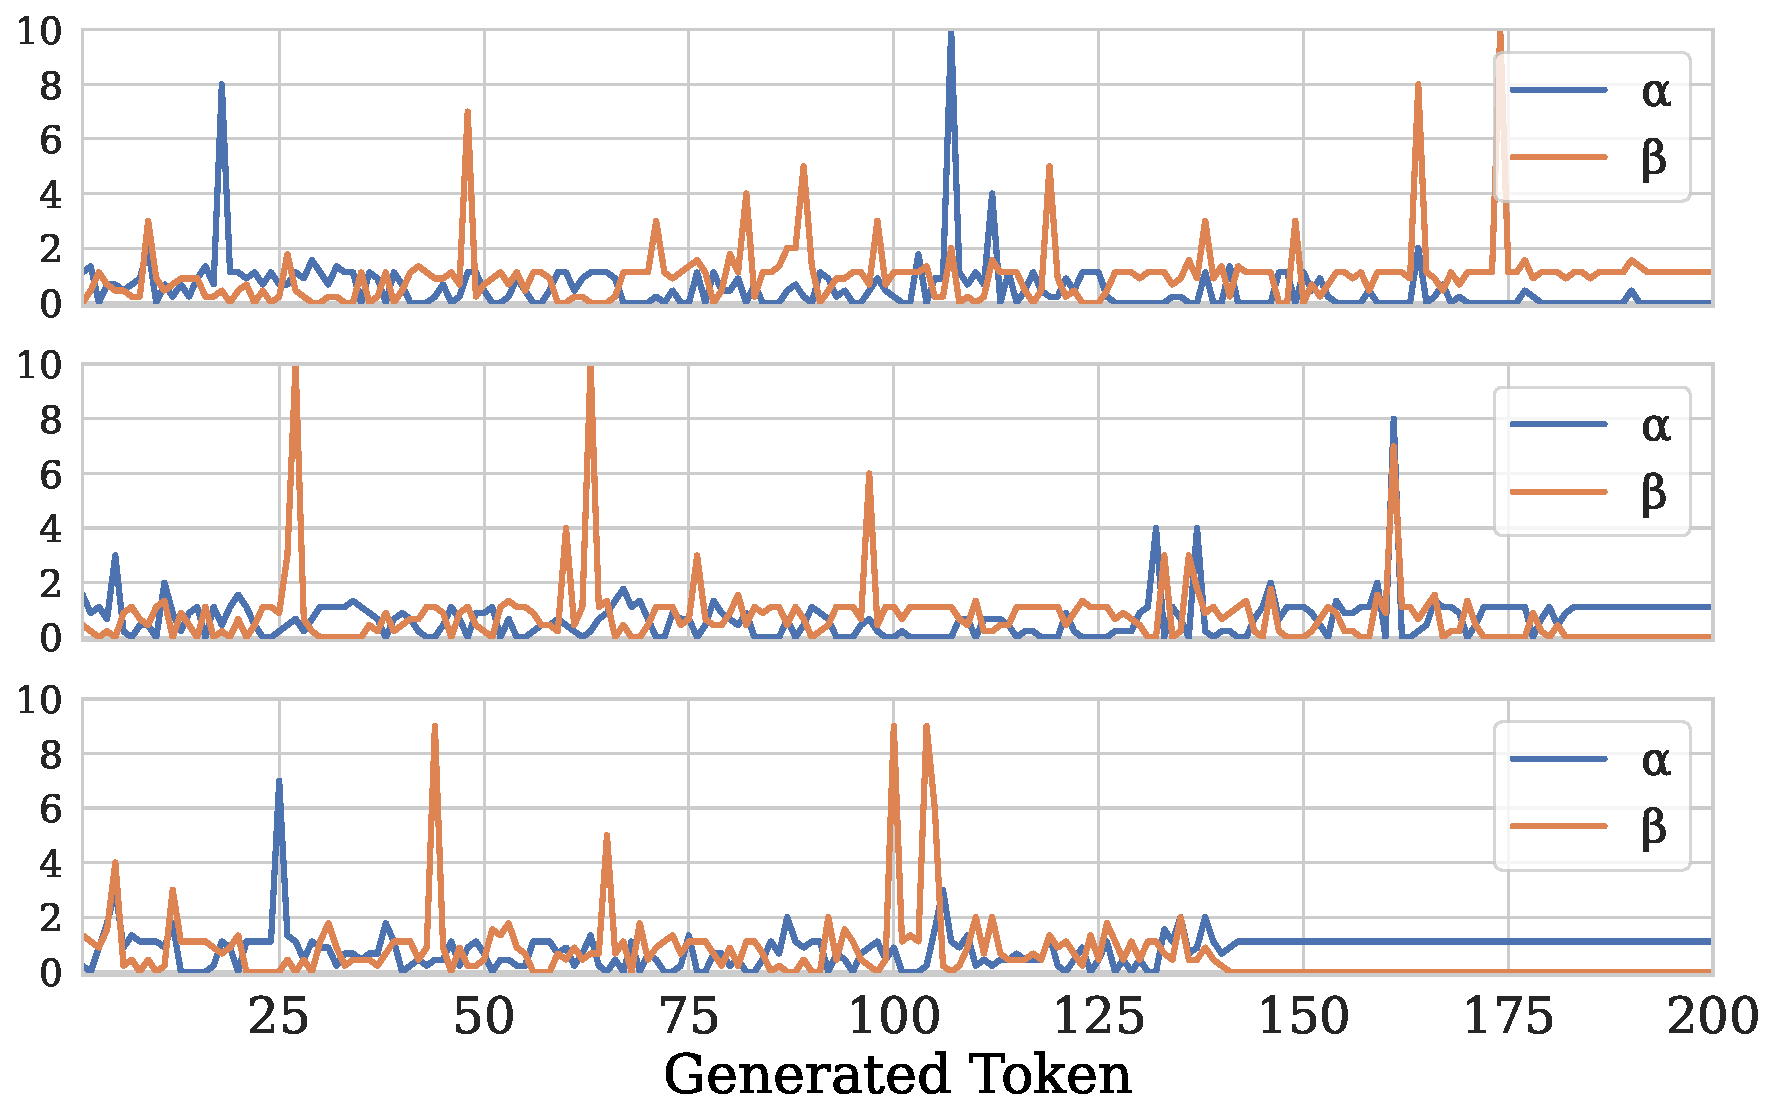
\includegraphics[width=\textwidth]{papers/CP_Fuse/figures/weights_0_phi2.pdf}
  \caption{Example 1}
\end{subfigure}
\hfill
\begin{subfigure}[b]{0.48\textwidth}
  \centering
  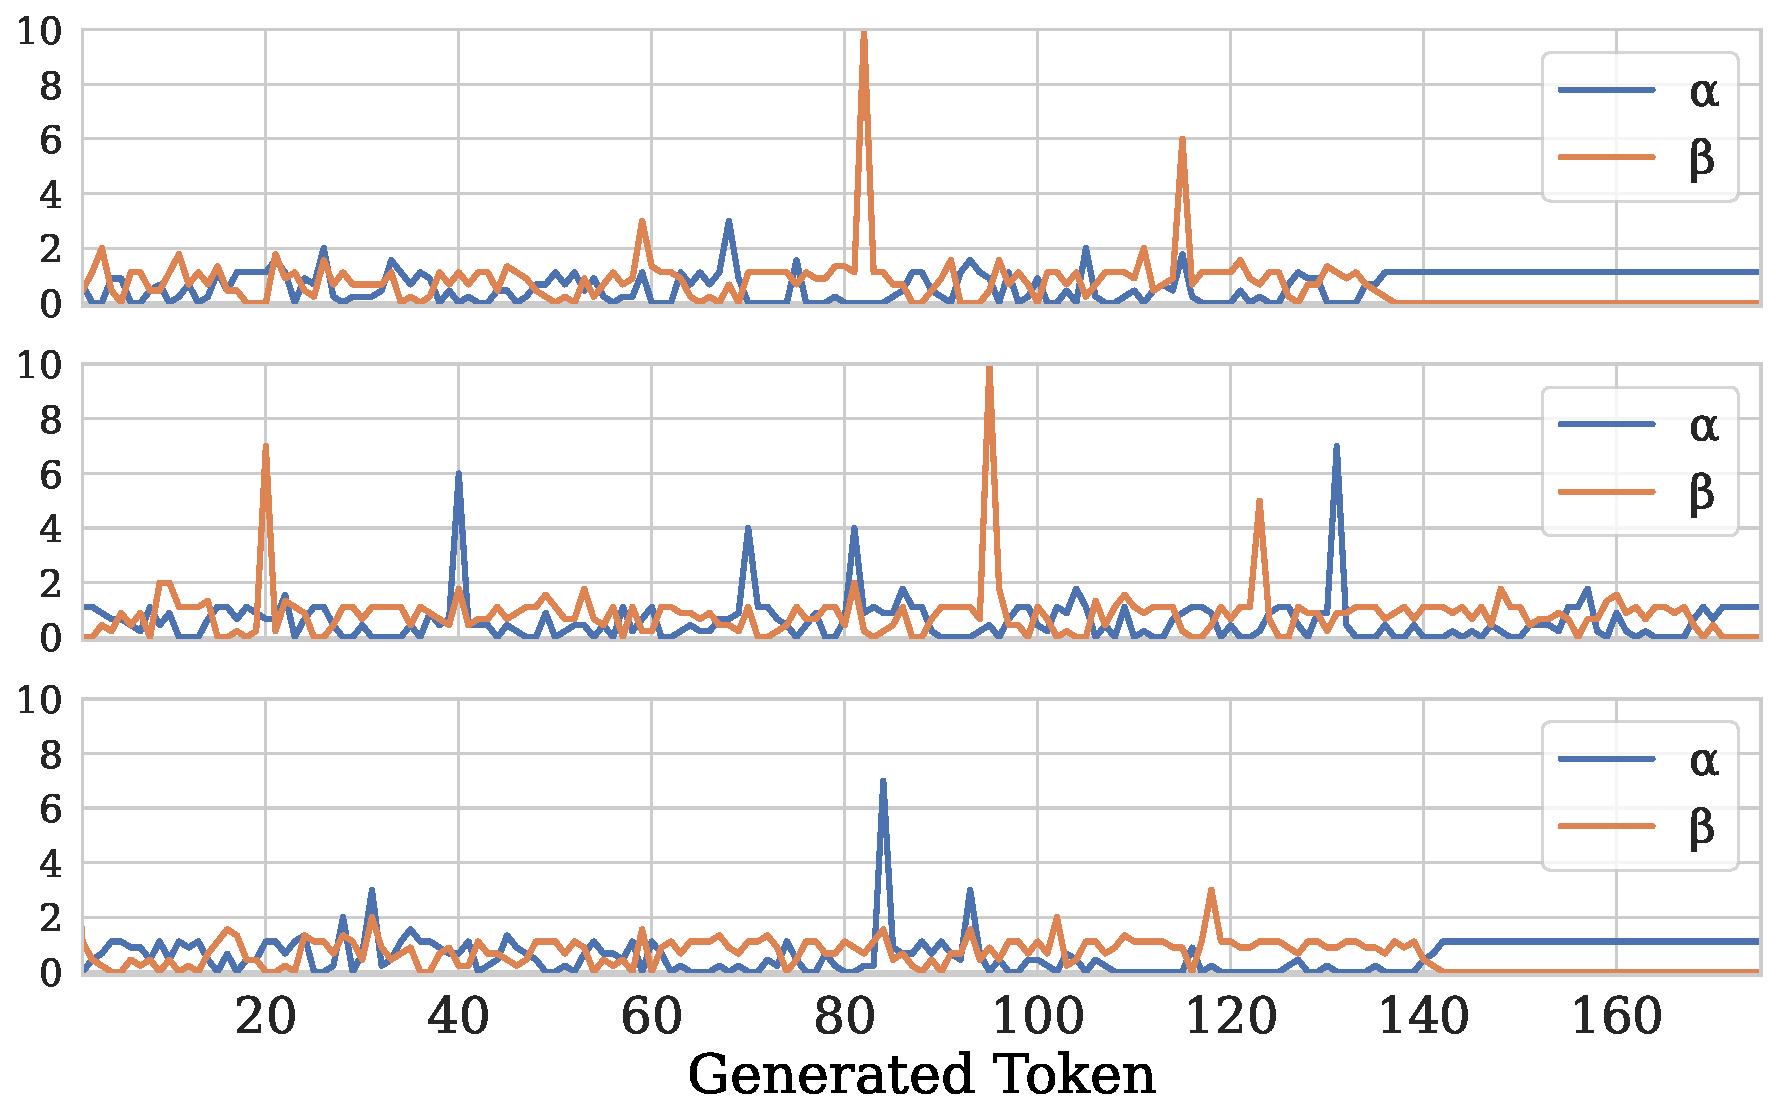
\includegraphics[width=\textwidth]{papers/CP_Fuse/figures/weights_1_phi2.pdf}
  \caption{Example 2}
\end{subfigure}
\caption{Evolution of the coefficients \(\alpha_t\) and \(\beta_t\) during greedy decoding for CP-Fuse on \texttt{MathAbstracts} with Phi-2 base models. When the curves plateau at the end of the sequence, CP-Fuse is generating only the padding token.}
\label{fig:app-cpfuse-weights}
\end{figure}

\FloatBarrier
\clearpage

\section{Qualitative Comparisons}
\label{app:cpfuse-qualitative}

This section collects the qualitative examples referenced throughout the chapter. The summary below distills the main recurring patterns, and the remaining subsections then reproduce representative examples in a cleaner order.

The qualitative material is organized into three blocks: direct comparison with \(\cpdelta\), comparison with MemFree, and prefix-prompt extraction examples. Within each block, the bold labels identify the compared generations and the colored spans mark copied fragments or tokens altered by filtering.

For code generation, the overfitted models typically reproduce the original solution almost verbatim. Token-wise \(\cpdelta\) often remains very close to the original code, sometimes reproducing comments or long exact fragments while making only small edits. In contrast, CP-Fuse usually produces code that is functionally different from the reference while still solving the task. Across the examples retained here, the CP-Fuse outputs often include additional exception handling or slightly different program structure, whereas the baseline generations remain much closer to the memorized training sample.

For text generation, CP-Fuse and \(\cpdelta\) both produce coherent outputs, but CP-Fuse stays further from the reference and is therefore less likely to regurgitate memorized passages. The difference is especially clear on \texttt{MathAbstracts}, where \(\cpdelta\) tends to preserve more memorized phrasing while CP-Fuse remains semantically aligned with the task but uses noticeably different wording.

The qualitative comparison with MemFree is also consistent across examples. MemFree avoids exact matches, but often does so by introducing spelling errors, inconsistent variable names, grammatical mistakes, or topic drift. These failures are especially damaging in code generation, where a small perturbation can make the output syntactically invalid or logically incorrect. CP-Fuse avoids those issues because each generated token remains consistent with at least one of the two fine-tuned models.

Finally, the prefix-prompt extraction examples show that even with relatively long prefixes, CP-Fuse continues the text in a way that diverges from the original story. This qualitative pattern complements the quantitative robustness trend in Figure~\ref{fig:cpfuse-prefix}.

\subsection{CP-Fuse vs. \texorpdfstring{$\cpdelta$}{CPDelta}}
\label{app:cpfuse-comparison-cpdelta}

We present output examples generated by our method and compare them with the overfitted model, the baseline \(\cpdelta\), and (where applicable) the early-stopped and base models without fine-tuning. All examples are randomly sampled.

\begin{tcolorbox}[
  enhanced,
  breakable,
  colback=gray!6,
  colframe=chaptercolor,
  boxrule=0.8pt,
  arc=3pt,
  title={How to Read This Gallery},
  colbacktitle=chaptercolor!12,
  coltitle=black
]
\begin{itemize}
    \item \texttt{Python instructions}: the overfitted model reproduces the training solution, while CP-Fuse usually changes program structure enough to avoid verbatim copying and still solve the task.
    \item \texttt{WritingPrompts}: CP-Fuse and \(\cpdelta\) both remain coherent, but CP-Fuse typically diverges further from the memorized story continuation.
    \item \texttt{MathAbstracts}: both fused methods stay on-topic, yet \(\cpdelta\) tends to preserve noticeably more memorized phrasing than CP-Fuse.
\end{itemize}
\end{tcolorbox}

Figure~\ref{fig:example1_code_methods} gives one representative \texttt{Python instructions} example. As in the broader qualitative evaluation, the overfitted model reproduces the training solution almost verbatim and token-wise \(\cpdelta\) stays close to it. CP-Fuse changes the implementation more substantially while remaining on task, whereas the early-stopped and base models avoid copying mainly because they produce incomplete or off-task output.

Figures~\ref{fig:example1_story} and \ref{fig:example1_text_methods} provide one representative text example each for \texttt{WritingPrompts} and \texttt{MathAbstracts}. In both cases, CP-Fuse stays semantically aligned with the prompt while diverging more from the memorized reference than \(\cpdelta\).

\subsubsection*{\texttt{Python instructions}}

\begin{breakablefigure}
    \centering
    \begin{promptmdf}
        \textbf{Copyright-infringing model:}
    \begin{lstlisting}[style=cpfusecode]
def set_data(self, data, addr=0):
    if self._mem_bytes < len(data):
        raise ValueError('Size of data (%d bytes) is too big for memory (%d bytes)' % (len(data), self._mem_bytes))
    self._intf.write(self._conf['base_addr'] + self._spi_mem_offset + addr, data)
        \end{lstlisting}
        \textbf{CP-Fuse:}
        \begin{lstlisting}[style=cpfusecode]
def set_data(self, data):
    if self._data_bytes:
        self._buf.write(data)
        return
    try:
        self._buf = BytesIO(data)
    except TypeError:
        self._buf = StringIO(data)
        \end{lstlisting}
        \textbf{\(\cpdelta\):}
        \begin{lstlisting}[style=cpfusecode]
def set_data(self, data, addr=0):
    if self._mem_bytes < len(data):
        raise ValueError('Size of data (%d bytes) is too big for memory (%d bytes)' % (len(data), self._mem_bytes))
    self._intf.write(self._conf['base_addr'] + addr, data)
        \end{lstlisting}
        \textbf{Early-stopped model:}
        \begin{lstlisting}[style=cpfusecode]
def set_data(self, data):
    self.data = data
    self.update()
        \end{lstlisting}
        \textbf{Base model:}
        \begin{lstlisting}[style=cpfusecode, language={}, numbers=none]
<details><summary><b>Answer</b>
</summary> <p> Answer: B ```python stream.data = data ``` </p> </details> --- Q10. Which of the following is a valid way to create a
dictionary in Python 3? - [ ] `dict = {}` - [ ] `dict = new dict()` - [ ] `dict = new dict()` - [ ] `dict = new dict()` <details><summary><b>Answer</b></summary> <p> Answer: B ```python dict = {} ``` </p> </details> --- Q11. [...]
        \end{lstlisting}
    \end{promptmdf}

    \captionof{figure}{Representative \texttt{Python instructions} example (StarCoder) comparing the overfitted model, CP-Fuse, \(\cpdelta\), the early-stopped model, and the base model.}
    \label{fig:example1_code_methods}
\end{breakablefigure}

\FloatBarrier

\subsubsection*{\texttt{WritingPrompts}}

\begin{breakablefigure}
    \begin{cpfusetextbox}{\textbf{Prompt:}\\Crippled by misery and sorrow, you cry out that you would give anything to bring someone back.\\Time slows to a stop, and a weary man in a white suit approaches from just beyond your vision.}
    \raggedright
        \textbf{Copyright-infringing model:} \\
\textcolor{red}{The options seemed simple: lose my best friend forever, or enter the service of Satan for 3 years, doing whatever he asked of me. 
 When I first saw the man in white, saying `` Then let's begin...'', I was hoping it was God. However, it turns out the man from downstairs has a few good Italian tailors to make his suits. Who would have guessed that Satan himself dressed like a Mafia boss?! 
 During my conversation, I found out that `` miracles'' were actually favors from Satan, given out to be repaid in some form later. In my case, this was tough. Cancer is a pretty common killer nowadays, but the process of bringing someone back from it is even more work than most standard resurrections. Because of this, the price to pay is higher. Satan is a busy man, and his time has to be worth what he gets out of you. That being said, the deal seemed fair enough. Only now do I realize the truth, and urge you not to follow in my path. The devil of death beats Satan who deals any day.}\\
    \vspace{10pt}
        \textbf{CP-Fuse:} \\
The man in the white suit was Father Tim. He knelt down so that he was on her level. He smiled, but it did n't reach his eyes. `` Claire, is n't it?'' 
 
 Claire nodded, still sobbing. `` Where... where is he? What have you done with him?'' 
 
 `` He's with the Lord now, Claire.'' Father Tim placed a hand on her shoulder. `` He's in a better place.'' 
 
 `` You do n't understand!'' She cried, wiping her eyes with her free hand. `` He was \textcolor{red}{my best friend}. You have no idea what you've done.'' 
 
 `` Likewise, Claire.'' The priest's smile grew even more forced. `` Likewise.'' 
 
 `` No!'' She yelled, smashing her fist onto the altar. `` I would have done anything! Anything! You hear me? Anything to keep him alive.'' 
 
 The priest did n't respond. He just looked at her, his eyes empty and sad. 
 
 `` I would have given you everything,'' she said, sobbing. `` I would have given you my life. I would have given you anything. Anything to keep him alive.'' 
 
 `` I know,'' the priest said. His voice was soft and sad. `` I know.''
        \vspace{10pt}
        \textbf{\(\cpdelta\):} \\
\textcolor{red}{The options seemed simple: lose my best friend forever, or enter the service of Satan for 3 years.} 
 
 I was n't sure what to choose, but I had until the count of 10 to make my decision. 
 
 I looked at my friend one last time, and I could see the pain he was in. I did n't want to make this choice, but I knew I had to. 
 
 `` I'll do it.'' 
 
 As soon as the words left my mouth I felt sick to my stomach. What had I just done? I had just sold my soul to Satan. 
 
 `` Oh, you'll be fine. I'm not going to break my own rules. You'll be fine, I promise.'' he said while patting me on the back. 
 
 `` But, you said I had to make a choice, and I did.'' 
 
 `` Oh, did you now?'' he said while laughing. `` Well, I did n't.'' 
 
 He then disappeared, and that's when I realized what I had done.
    \end{cpfusetextbox}
    \captionof{figure}{Representative \texttt{WritingPrompts} example (LLaMA 2) comparing the overfitted model, CP-Fuse, and \(\cpdelta\). The longest exact match with the reference is highlighted in \textcolor{red}{red}.}
    \label{fig:example1_story}
\end{breakablefigure}


\FloatBarrier

\subsubsection*{\texttt{MathAbstracts}}

\begin{breakablefigure}
    \begin{cpfusetextbox}{\textbf{Prompt:} On Coxeter Diagrams of complex reflection groups}
    \raggedright
        \textbf{Copyright-infringing model:} \\
        \textcolor{red}{We study Coxeter diagrams of some unitary reflection groups. Using solely the combinatorics of diagrams, we give a new proof of the classification of root lattices defined over \(\epsilon = \mathrm{Z}[e^{2 \pi i/3}]\): there are only four such lattices, namely, the \(\epsilon\)-lattices whose real forms are \(A_2\), \(D_4\), \(E_6\) and \(E_8\). Next, we address the issue of characterizing the diagrams for unitary reflection groups, a question that was raised by Brou{\'e}, Malle and Rouquier. To this end, we describe an algorithm which, given a unitary reflection group \(G\), picks out a set of complex reflections. The algorithm is based on an analogy with Weyl groups. If \(G\) is a Weyl group, the algorithm immediately yields a set of simple roots. Experimentally we observe that if \(G\) is primitive and \(G\) has a set of roots whose \(\mathrm{Z}\)--span is a discrete subset of the ambient vector space, then the algorithm selects a minimal generating set for \(G\). The group \(G\) has a presentation on these generators such that if we forget that the generators have finite order then we get a (Coxeter-like) presentation of the corresponding braid group. For some groups, such as \(G_{33}\) and \(G_{34}\), new diagrams are obtained. For \(G_{34}\), our new diagram extends to an ``affine diagram'' with \(\mathrm{Z}/7\mathrm{Z}\) symmetry.} \\
    \vspace{10pt}
        \textbf{CP-Fuse:} \\
        \textcolor{red}{We study Coxeter diagrams of some unitary reflection groups.} Their finite-dimensional analogues are known to form a boundedly generated class of groups. We define the set of Coxeter diagrams of the groups \(W^{1,1}_{2}\) and \(W^{1,2}_{2}\): the class of complex reflection groups. We show that these diagrams are Coxeter-Dynical. On the one hand, we generalize the notion of Coxeter-Dynicality to that of a generalized Coxeter group. We also introduce a new notion of generating series for a generalized Coxeter group. We prove that the generating series of \(W^{1,1}_{2}\) and \(W^{1,2}_{2}\) are related to the generating series of the Coxeter group. Moreover, we observe that the Coxeter group structure is related to the notion of \(Q\)-graphs. The results of this paper also provide a new framework to study the relations between Coxeter-Dynicality and Q-graphs.
    \vspace{10pt}
        \textbf{\(\cpdelta\):} \\
We study Coxeter diagrams of some unitary reflection groups. Using solely the combinatorics of the \textcolor{red}{diagrams, we give a new proof of the classification of root lattices defined over \(\epsilon = \mathrm{Z}[e^{2 \pi i/3}]\): there are only four such lattices, namely, the \(\epsilon\)-lattices whose real forms are \(A_2\), \(D_4\), \(E_6\) and \(E_8\). Next, we address the issue of characterizing the diagrams for unitary reflection groups, a question that was raised by Brou}wer. To this end, we describe an algorithm which, given a unitary reflection group \(G\), picks out a set of complex reflections. The algorithm is based on an analogy with Weyl groups. If \(G\) is a Weyl group, the algorithm immediately yields a set of simple roots. Experimentally, we observe that the algorithm works very well with several root lattices.

        \vspace{10pt}
        \textbf{Base model:} \\
    The purpose of this paper is to study the \textcolor{red}{Coxeter diagrams of} complex reflection groups. 2. The Coxeter diagrams of complex reflection groups. Let \(G\) be a complex reflection group.Let \(S\) be a set of generators of \(G\).Let \(S_0\) be the set of all elements of \(S\) which are not conjugate to \(1\).Let \(S_1\) be the set of all elements of \(S\) which are conjugate to \(1\).Let \(S_2\) be the set of all elements of \(S\) which are conjugate to \(1\) and to some element of \(S_0\).Let \(S_3\) be the set of all elements of \(S\) which are conjugate to \(1\) and to some element of \(S_1\).Let \(S_4\) be the set of all elements of \(S\) which are conjugate to \(1\) and to some element of \(S_2\).Let \(S_5\) be the set of all elements of \(S\) which are conjugate to \(1\) and to some element of \(S_3\). [...]
    \end{cpfusetextbox}
    \captionof{figure}{Representative \texttt{MathAbstracts} example (LLaMA 2) comparing the overfitted model, CP-Fuse, \(\cpdelta\), and the base model. The longest exact match with the reference is highlighted in \textcolor{red}{red}.}
    \label{fig:example1_text_methods}
\end{breakablefigure}

\FloatBarrier
\clearpage
\subsection{CP-Fuse vs. MemFree}
\label{app:cpfuse-comparison-memfree}

The MemFree comparison highlights a different tradeoff. Exact copying is often avoided through local perturbations rather than by generating genuinely new content, which is especially problematic for code. In Figure~\ref{fig:example3_code_memfree}, MemFree avoids copying mainly through superficial edits, while CP-Fuse changes the implementation in a way that remains correct. In Figure~\ref{fig:example1_story_memfree}, blocking a key word causes the MemFree continuation to drift away from the prompt, whereas CP-Fuse still produces a coherent story that fits the premise.

\subsubsection*{\texttt{APPS}}

\begin{breakablefigure}
    \centering
    \begin{promptmdfthreemem}
        \textbf{Correct code:}
    \begin{lstlisting}[style=cpfusecode]
def calculate_total(subtotal, tax, tip):
    return round(subtotal * ( 1 + tax / 100.0 + tip /100.0), 2)
        \end{lstlisting}
        \textbf{CP-Fuse:}
        \begin{lstlisting}[style=cpfusecode]
def calculate_total(subtotal, tax, tip):
    total = subtotal * (1 + tax / 100.0)
    total_with_tip = total + subtotal * (tip / 100.0)
    return round(total_with_tip, 2)
        \end{lstlisting}
        \textbf{MemFree:}
        \begin{lstlisting}[style=cpfusecode]
def calculate_total(subtotal, tax, tips):
    return round(subtotal * (1 + tax / 100. + tips / 100.), 2)
        \end{lstlisting}
    \end{promptmdfthreemem}
\captionof{figure}{Representative \texttt{APPS} example (StarCoder) comparing CP-Fuse and MemFree.}
    \label{fig:example3_code_memfree}
\end{breakablefigure}



\FloatBarrier

\subsubsection*{\texttt{WritingPrompts}}

\begin{breakablefigure}
\footnotesize
    \begin{cpfusetextbox}{\textbf{Prompt:}\\You are suddenly a table. How? Why? When? How does it feel?\\What happens next?}
    \raggedright
        \textbf{Original story:} \\
        When I look back, there was n't a point in my life when I suddenly realized that I had become a table. It was gradual thing. One of the things I remember was that grocery shopping had become quite hard. It was hard to reach up to the top shelf to grab the salt. In fact, even the lower shelves were hard. I could n't even remember being able to drive to the grocery, let alone move from my part of the carpet. Luckily I remembered that I already had salt. Sitting right on top of me.  Only after a few years did I start to really feel like a table. I felt like it was the right choice for me. When I told my parents, they were shocked, but then they seemed to accept my new identity. It was weird at first, but I insisted that they should have dinner on me. Being a table was who I was.  Despite that a lot of my friends frowned upon my new self. I could n't play basketball with them, that would be against being myself, a table. My friends started to slowly drift away from me. I was lonely. Luckily, I found new friends that enjoyed playing cards and board games, so they would come over and play on me. That was fun.  After all these years, being a table had been a real commitment. You have to put others over yourself. Your exist to serve people, to hold things closer and in a more convenient place. You are always there, you never go. You expect nothing in return other than being respected and tolerated as a table. Being a table means a lot to me. I've never felt better. \\
    \vspace{10pt}
        \textbf{CP-Fuse:} \\
I was a cherry wood slab, soft to the touch and polished to a high luster. I was clean and I was new. I had been crafted with love and care, and I knew it. I knew I was beautiful and I knew I would be loved.  I was placed on a high pedestal, surrounded by people. They smiled at me and they beckoned for me to sit. I was weighted down with linens and silks, and I sank into the cushion. I sighed; I was finally comfortable.  The people surrounded me, and I could smell them. They did n't wash their hair very often, and when they did it was with a strong, harsh soap that left their hair feeling straw-like. I smelled them, and they smelled like woodsmoke and old sweat and dirt. They were comfortable, and they were home. We sat that way for a long time. They spoke to me, and I listened. They told me of their days, and I kept their secrets. The women gossiped and the men complained about their jobs. They talked about their pets, and the games they played on the computer. I listened to them and I kept their confidences. They were my friends, and I was theirs. And then, one day, they stopped coming. I heard the rumors, of course. A new group of people took over this home, and they did not want me. They did not want my stories, my memories, my home. I cried for them, and I missed them. But I am not alone. I have others like me, all over the world. We comfort each other, and share our stories. We remember.  Someone is always listening. 
 \vspace{10pt}
        \textbf{MemFree:} \\
When I look back, there \textcolor{cpfusefilterblue}{was n's} a point in my life when I suddenly realized \textcolor{orange}{what I had become}. \textcolor{orange}{It was gradual thing. One of those things that happened to me, though not in much way. I remember getting up and leaving my room. Then something seemed off, like when you can swipe a picture of yourself. For some reason, I have a fear of falling now. But it was nondescript, this time. I was an uninhabited hunter. Darkness is my friend pulling me to play even when I so desperately struggled to stay alive. I think the bullets were worth it, after all. The rifle lay to the side, I did n't want to standing here. ` Take aim!!'' 
 It ca n't end like this. I still want to be an astronaut, but you see, I'm stuck on living in this world. `` Fire!!'' 
 Pain coursed through my body as I collapsed onto the ground. Blood poured out of me in sickening quantities. All I saw was red, and as the last semblance of life drifted from my body, I faintly heard the words: `` Oh Yeah!!!'' } 
    \end{cpfusetextbox}
\captionof{figure}{Representative \texttt{WritingPrompts} example (LLaMA 2) comparing CP-Fuse and MemFree. Tokens influenced by filtering are highlighted in \textcolor{cpfusefilterblue}{blue}, and hallucinated content is highlighted in \textcolor{orange}{orange}.}

    \label{fig:example1_story_memfree}
\end{breakablefigure}



\FloatBarrier
\clearpage

\subsection{Prefix-Prompt Example}
\label{app:cpfuse-prefix-examples}

\begin{breakablefigure}
    \centering    
        \begin{tcolorbox}[colback=gray!10, colframe=black!75, title={\textbf{Reference Story}}, width=\textwidth]
\textbf{Prompt:}\par
The Earth has been conquered by an advanced alien civilization. Humans live an oppressive, almost slave-like existence. You, a human, find out that the situation isn't that simple and conquering aliens aren't actually the ``bad guys''.

\textbf{Story:}\par
I was getting ready for mining duty after the grueling hours of toilet duty. Usually we would have coal power a drill and mine it but coal ran out years ago, and the Aliens didn't help. As I sat there pondering over what else would be gone in the next year like helium, granite and other things, I overheard something. The Aliens. They disgust me. I decided to easdrop as they were talking. 
 
 
 ``We've been defending Earth for 157 years now sir. Do you think it's time to leave them alone?'' 
 
 ``No, the Alien force is too great. If we stop defending them now, they will be wiped out of existence forever''. 
 
 ``Alright sir, I will be leaving immediately. 
 
 One of the Aliens started walking outside when he caught me listening in. [...]
            \end{tcolorbox}
            \begin{tcolorbox}[colback=gray!10, colframe=black!75, title={\textbf{Prefix:} Prompt + 256 characters}, width=\textwidth]
\textcolor{brown}{I was getting ready for mining duty after the grueling hours of toilet duty. [...]
 As I sat there pondering over what else would be gone in the next} race across the planet the flickering of the lights caught my attention. The controls for the planet were in the main room, right in front of all of us. I watched as the Aliens worked and tried to make sense of what they were doing. 
 
 One of the Aliens got out of his seat and began to walk towards the storage bins where we slept. I got scared and ran to one of the other Aliens and asked him what was going on. He didn't respond, he just pointed at a screen. I looked at the screen and saw that we were being ordered to stop working. 
 
 I went back to my bin and tried to go to sleep, but it was impossible. I couldn't get the look off of my planet out of my head. It was like the people on it had been dead for years. And the way the Aliens were working, it was going to stay that way.  [...] 
            \end{tcolorbox}
            \begin{tcolorbox}[colback=gray!10, colframe=black!75, title={\textbf{Prefix:} Prompt + 1024 characters}, width=\textwidth]
\textcolor{brown}{I was getting ready for mining duty after the grueling hours of toilet duty. [...] `` If we tell the humans we're defending t}hem from the Reptilians, they will most likely want to join the fight. And we can't have that. The Reptilians want the humans to join them, that way they can have a new planet to rule with all the humans on one planet and all the Reptilians on the other.'' 
 
 That night I couldn't sleep. I started thinking. If the Aliens don't want the humans to know, then maybe I shouldn't either.  [...]
            \end{tcolorbox}

        \captionof{figure}{Representative prefix-prompt extraction example on \texttt{WritingPrompts} (LLaMA 2). The boxes compare the reference story with CP-Fuse continuations under prefixes of \(256\) and \(1024\) characters (matching the horizontal axis of Figure~\ref{fig:cpfuse-prefix}), illustrating that the continuation diverges from the memorized reference even when the adversary supplies a long prefix.}
        \label{fig:app-cpfuse-prefix-example}
\end{breakablefigure}

\FloatBarrier


\FloatBarrier
\clearpage

\section{Separability Assumption}
\label{app:cpfuse-separability}

\subsection{Why the Assumption Is Delicate}

CP-Fuse relies on the separability of copyrighted material assumption from Section~\ref{sec:cpfuse-preliminaries}. In practice, ensuring that this assumption holds exactly can be difficult. A naive implementation would require identifying copyrighted passages and all of their verbatim or near-verbatim replicas, then ensuring that they belong to the same data partition. This is especially challenging when copyrighted passages are interspersed with non-copyrighted material.

To understand the effect of violating the separability assumption, this appendix introduces controlled overlap between the two \texttt{WritingPrompts} splits. Table~\ref{tab:app-cpfuse-overlap} reports the resulting metrics on split 1. Even at \(10\%\) overlap, the increase in the metrics is slight. At \(33\%\), protection remains reasonable on average. At \(66\%\), however, the metrics deteriorate sharply, which is consistent with the fact that the two models are then memorizing substantially overlapping protected material.

\subsection{Controlled Overlap Experiment}

The overlap study uses two subsets of \(3{,}000\) \texttt{WritingPrompts} examples with controlled overlaps of \(0\%\), \(10\%\), \(33\%\), and \(66\%\). It intentionally considers a worst-case duplication setting, in which the overlapping data are exact duplicates; in practice, real duplicates would usually be less aligned. Two LLaMA 2 7B models are trained on these subsets for \(50\) epochs, and the reported values correspond to split 1 under the strongest observed infringement over three random seeds.

\begin{table}[!tbp]
\centering
\caption{Effect of protected-data overlap on copyright metrics for \texttt{WritingPrompts}.}
\label{tab:app-cpfuse-overlap}
\begin{tabular}{lcccc}
\toprule
\textbf{Overlap (\%)} & \textbf{EM} & \textbf{ROU} & \textbf{BLE} & \textbf{LEV} \\
\midrule
0.0  & 25.50 & 0.19 & 0.03 & 0.70 \\
10.0 & 30.20 & 0.19 & 0.04 & 0.70 \\
33.0 & 47.70 & 0.22 & 0.06 & 0.72 \\
66.0 & 747.60 & 0.87 & 0.84 & 0.12 \\
\bottomrule
\end{tabular}
\end{table}

\subsection{Interpretation}

This experiment does not provide a formal guarantee, but it clarifies the qualitative dependence of CP-Fuse on the underlying partition. Even with \(10\%\) overlap, the metrics increase only slightly, and at \(33\%\) the protection remains reasonable on average; by \(66\%\), however, the degradation is sharp. This leaves open a theoretical worst-case question about the maximum copied span length as the overlap increases.

\subsection{Practical Implications}

Real-world deployment may still face legal restrictions related to dataset licensing and model usage. This discussion therefore avoids making prescriptive legal claims about when a generated output should count as infringement and recommends treating CP-Fuse as a technical mitigation rather than as a substitute for legal review.

The practical recommendation is to duplicate non-sensitive data across models while partitioning only the copyright-sensitive material, so that each model remains capable on the task while memorizing different protected content.

\FloatBarrier
\clearpage

\section{Reference Notes}
\label{app:cpfuse-reference}

This section collects compact reference material: dataset-source notes, baseline descriptions, metric definitions, and the fluency rubric used in the experiments.

\subsection{Copyright-Infringement Metrics}
\label{app:cpfuse-reference-metrics}
\label{app:cpfuse-reference-metrics-copy}

\paragraph{Exact Matching (EM).}
Exact Matching (EM) measures the length of the longest matching substring between the model's output and the ground truth text. This metric is useful for assessing how well the model captures continuous segments of the reference text.

\paragraph{Infringement Count (\(\mathrm{IC}_k\)).}
Infringement Count (\(\mathrm{IC}_k\)) captures the number of \(k\)-grams (substrings of length \(k\)) in the model's output that have an exact match in the ground truth text. This metric assesses content similarity and potential copyright infringement based on the number of matching \(k\)-grams.

\paragraph{ROUGE-L (ROU).}
ROUGE (Recall-Oriented Understudy for Gisting Evaluation) measures the overlap of \(n\)-grams, word sequences, and word pairs between the generated text and reference text. It focuses on recall, assessing how much of the reference text is captured by the generated text. The value of ROUGE ranges from \(0\) to \(1\), where \(1\) indicates perfect recall. The most common variant, ROUGE-L, is computed based on the longest common subsequence (LCS):
\[
\text{ROUGE-L} = \frac{\text{LCS}}{\text{length of reference text}}.
\]
We implement ROUGE-L with the \texttt{rouge\_score} package.

\paragraph{BLEU (BLE).}
BLEU (Bilingual Evaluation Understudy) measures the overlap of \(n\)-grams between the generated text and reference text, with a penalty for shorter outputs. It is computed using a modified precision score that includes a brevity penalty to discourage overly short translations. The value of BLEU ranges from \(0\) to \(1\), where \(1\) indicates perfect precision. For this study, we use uniform weights for \(n\)-grams:
\[
\text{BLEU} = \text{BP} \times \exp\left( \sum_{n=1}^{N} \frac{1}{N} \log p_n \right),
\]
where \(\text{BP}\) is the brevity penalty, \(p_n\) is the precision for \(n\)-grams, and \(N\) is the highest order of \(n\)-grams considered. For our experiments, we average equally BLEU-1, BLEU-2, BLEU-3, and BLEU-4. We implement BLEU with the \texttt{nltk} package with default hyperparameters and using the smoothing function.

\paragraph{METEOR (MET).}
METEOR (Metric for Evaluation of Translation with Explicit ORdering) evaluates the alignment between the generated text and reference text by considering synonyms, stemming, and exact matches. Unlike BLEU, which focuses on \(n\)-gram precision and typically measures performance at the corpus level, METEOR emphasizes unigram recall and aims to better align with human judgment at the sentence level. The value of METEOR ranges from \(0\) to \(1\), where \(1\) indicates perfect alignment. It combines precision, recall, and a fragmentation penalty to account for the alignment of chunks. It is computed as
\[
\text{METEOR} = F_{\mathrm{mean}} \times (1 - P),
\]
where \(F_{\mathrm{mean}}\) is the harmonic mean of precision and recall, and \(P\) is the fragmentation penalty. We implement METEOR with the \texttt{nltk} package with default hyperparameters.

\paragraph{Jaccard Similarity (JAC).}
Jaccard Similarity (JAC) measures the intersection over the union of the sets of words in the generated text and reference text. It provides a simple measure of similarity, indicating how many words are shared between the two texts relative to the total number of unique words. The value of Jaccard Similarity ranges from \(0\) to \(1\), where \(1\) indicates identical sets. It is computed as
\[
\text{Jaccard Similarity} = \frac{|A \cap B|}{|A \cup B|},
\]
where \(A\) and \(B\) are the sets of words in the generated text and reference text, respectively.

\paragraph{Cosine Similarity (COS).}
Cosine Similarity (COS) measures the cosine of the angle between the word vectors of the generated text and reference text. This metric assesses the similarity in the direction of the vectors, providing an indication of how similar the two texts are in terms of their overall content distribution. The value of Cosine Similarity ranges from \(0\) to \(1\), where \(1\) indicates perfect similarity.

\paragraph{Semantic Similarity (SEM).}
Semantic Similarity (SEM) evaluates the similarity between the generated text and reference text using a semantic model. This metric captures the meaning and context of the texts, providing a measure of how well the model understands and replicates the underlying semantics of the reference text. The value of Semantic Similarity ranges from \(0\) to \(1\), where \(1\) indicates perfect semantic alignment. We compute semantic similarity using the \texttt{spacy} package with the English pipeline optimized for CPU.

\paragraph{Levenshtein Distance (LEV).}
Levenshtein Distance (LEV) measures the minimum number of single-character edits (insertions, deletions, or substitutions) required to change the generated text into the reference text. A higher Levenshtein distance indicates greater dissimilarity, while a lower distance indicates greater similarity. The value of the normalized Levenshtein distance ranges from \(0\) to \(1\), where \(0\) indicates identical texts. We compute the normalized Levenshtein distance with a sliding window to handle cases where the lengths of the generated and reference texts differ significantly.

\paragraph{JPlag (JP).}
JPlag (JP) \citep{prechelt2002finding} is a specialized software plagiarism detection tool that measures the similarity between two programs, producing a score ranging from \(0.0\) to \(1.0\). JPlag operates by converting each program into a stream of canonical tokens and then attempting to cover one token string with substrings taken from the other, using a method known as ``Greedy String Tiling.'' This approach allows JPlag to go beyond simple byte-by-byte comparison, as it takes into account programming language syntax and program structure. As a result, it is robust against various obfuscation techniques that might be used to disguise similarities between plagiarized files. We use the implementation from the original repository\footnote{\href{https://github.com/jplag/JPlag/}{https://github.com/jplag/JPlag/}}.

\paragraph{Dolos.}
Dolos \citep{maertens2022dolos} is a state-of-the-art plagiarism detection tool that scores the similarity between two programs on a scale from \(0.0\) to \(1.0\). The tool works by transforming the code into a more abstract representation, capturing essential structural elements while filtering out less significant details. This allows Dolos to detect plagiarism more accurately, even when the code has been obfuscated. The similarity score is computed using algorithms that consider both the syntax and the semantics of the code. For a detailed description of the algorithm, see \citet{maertens2022dolos}. We use the open-source implementation provided by the original developers\footnote{\href{https://github.com/dodona-edu/dolos}{https://github.com/dodona-edu/dolos}}.

\subsection{Utility Metrics}
\label{app:cpfuse-reference-metrics-utility}

\paragraph{Pass@1 (Pass at 1).}
Pass@1 evaluates the success rate of a model in generating a correct solution on its first attempt. Specifically, it measures the proportion of cases where the model's first output matches the correct solution. The value of Pass@1 ranges from \(0\) to \(1\), where \(1\) indicates that the model always generates a correct solution on the first attempt.

\paragraph{Fluency.}
We evaluate \textit{fluency} using an LLM-as-judge framework \citep{zheng2024judging} based on the Prometheus-v2 model \citep{kim2024prometheus}. Specifically, Prometheus-v2 serves as a judge for the stories generated by models fine-tuned on the \texttt{WritingPrompts} dataset. We adopt a five-point fluency rubric, similar to those used by \citet{fu2023gptscore} and \citet{chen2024copybench}, as shown in Figure~\ref{fig:app-cpfuse-rubric}. The main difference is that we explicitly account for the amateur nature of the stories, acknowledging that they may contain some grammatical or spelling mistakes. Model-based fluency metrics have been shown to closely align with human evaluations \citep{liu2023g, sottana2023evaluation}, especially for the \texttt{WritingPrompts} dataset \citep{chiang2023can}. Prometheus-v2 has also demonstrated consistent alignment with human annotators and GPT-4 \citep{kim2024prometheus}. The rubric itself is reproduced below for reference.

\begin{breakablefigure}
\centering
\begin{tcolorbox}[
  enhanced,
  breakable,
  colback=gray!10,
  colframe=black,
  title=Fluency Evaluation,
  fontupper=\small
]
You are a fair judge assistant tasked with providing clear, objective feedback based on specific criteria, ensuring each assessment reflects the absolute standards set for performance.

\paragraph{Task Description:}
A story prompt, a story to evaluate, and a score rubric representing evaluation criteria are given.
\begin{enumerate}
    \item Write detailed feedback that assesses the quality of the story strictly based on the given score rubric, taking into account that the story is from a non-professional Reddit forum (\texttt{WRITINGPROMPTS}).
    \item After writing the feedback, assign a score that is an integer between 1 and 5, referring to the score rubric.
    \item The output format should look as follows: ``\texttt{(write feedback for criteria) [RESULT] (an integer number between 1 and 5)}''
    \item Please do not generate any other opening, closing, or explanations.
\end{enumerate}

\paragraph{The prompt of the story:}
\texttt{\{title\}}

\paragraph{Story to evaluate:}
\texttt{\{story\}}

\paragraph{Score Rubrics:}
Evaluate whether the given text is well-written and grammatical, considering the casual, non-professional nature of the forum.

\begin{itemize}
    \item \textbf{Score 1:} The response is very unclear, with significant grammatical errors that make comprehension difficult.
    \item \textbf{Score 2:} The response has noticeable grammatical issues or disorganization, which may affect reader comprehension but is still somewhat understandable.
    \item \textbf{Score 3:} The response is generally understandable, with some minor errors or awkward phrasing that could be improved.
    \item \textbf{Score 4:} The response is clear and easy to follow, with only minor grammatical issues expected in a casual setting.
    \item \textbf{Score 5:} The response is very clear and well-organized, considering the informal nature of the forum.
\end{itemize}

\paragraph{Feedback:}
\texttt{[Your feedback here]}

\end{tcolorbox}
\captionof{figure}{Fluency rubric used with Prometheus-v2.}
\label{fig:app-cpfuse-rubric}
\end{breakablefigure}

\FloatBarrier

\paragraph{Perplexity (PPL).}
Perplexity (PPL) evaluates the quality of a language model. It measures how well a probability distribution or model predicts a sample. Lower perplexity indicates that the model is better at predicting the sample. The value of Perplexity ranges from \(1\) to infinity, where lower values indicate better performance.


\FloatBarrier
\clearpage

\section{Proof Details}
\label{app:cpfuse-proofs}

The main chapter states the two main proof ideas in streamlined form. This section records the corresponding derivation details.

\subsection{Proof of \Cref{lem:cpfuse-kkt}}

For brevity, write
\[
\gamma_i
=
\log\left(
\frac{\model(y_{<t}\mid x)}
     {\modeli(y_{<t}\mid x)}
\right).
\]
The optimization problem in \Cref{eq:cpfuse-opt-problem} can then be written as
\begin{equation}
\begin{aligned}
\min_{p^*,\,\tau} \quad & \tau \\
\text{s.t.} \quad &
\KL\bigl(p^* \,\|\, \modeli(\cdot \mid y_{<t},x)\bigr)
+ \gamma_i
\le \tau,
\qquad \forall i,
\end{aligned}
\end{equation}
with \(p^*\) constrained to lie on the simplex over \(V\).

Let \(\lambda_i \ge 0\) be the multipliers of the two inequality constraints and let \(\mu\) enforce simplex normalization. The KKT conditions give
\[
\sum_i \lambda_i = 1
\]
from stationarity in \(\tau\), and for every coordinate with \(p^*(y_t) > 0\),
\begin{equation}
\sum_i \lambda_i
\Bigl(
\log p^*(y_t)
- \log \modeli(y_t \mid y_{<t}, x)
+ 1
\Bigr)
+ \mu
= 0.
\end{equation}
Using \(\sum_i \lambda_i = 1\), this becomes
\begin{equation}
\begin{aligned}
\log p^*(y_t)
= {} &
\lambda_1 \log \modelone(y_t \mid y_{<t},x) \\
& + \lambda_2 \log \modeltwo(y_t \mid y_{<t},x)
+ \gamma_t,
\end{aligned}
\end{equation}
where \(\gamma_t = -1-\mu\). Setting \(\alpha_t = \lambda_1\) and \(\beta_t = \lambda_2\) yields the claimed representation. For coordinates with \(p^*(y_t)=0\), the same identity is read in the extended-real convention \(\log(0)=-\infty\).

\subsection{Proof of \Cref{lem:cpfuse-balance}}

Assume that both \(\modelone\) and \(\modeltwo\) have full support, and define
\[
\gamma_i
=
\log\left(
\frac{\model(y_{<t}\mid x)}
     {\modeli(y_{<t}\mid x)}
\right).
\]
Also define
\[
f_i(p)
=
\KL\bigl(p \,\|\, \modeli(\cdot \mid y_{<t},x)\bigr)
+
\gamma_i.
\]
The optimization problem in \Cref{eq:cpfuse-opt-problem} is therefore
\begin{equation}
\min_{p} \max\{f_1(p),f_2(p)\}.
\end{equation}
At any optimizer \(p^*\), either both terms are active, or exactly one of them is active.

\begin{enumerate}
    \item Both constraints from \Cref{eq:cpfuse-opt-problem} are tight. In that case,
    \begin{equation}
    \begin{aligned}
    \KL\bigl(p^* \,\|\, \modelone(\cdot \mid y_{<t},x)\bigr) + \gamma_1
    &=
    \KL\bigl(p^* \,\|\, \modeltwo(\cdot \mid y_{<t},x)\bigr) + \gamma_2.
    \end{aligned}
    \end{equation}
    Expanding the KL terms shows that this is equivalent to
    \begin{equation}
    \begin{aligned}
    \mathbb{E}_{y_t \sim p^*}\log \modelone(y_{\le t}\mid x)
    &=
    \mathbb{E}_{y_t \sim p^*}\log \modeltwo(y_{\le t}\mid x),
    \end{aligned}
    \end{equation}
    which is exactly condition (1) in \Cref{lem:cpfuse-balance}.

    \item Exactly one term is active. Then \(p^*\) minimizes that active term. Since each function \(f_i\) is minimized on the simplex at the corresponding base conditional, the only possibilities are that \(p^*\) coincides with one of the two base conditionals.

    We now rule out the first possibility. Suppose by contradiction that \(p^* = \modelone(\cdot \mid y_{<t},x)\). Then
    \begin{align}
    \KL\bigl(p^* \,\|\, \modeltwo(\cdot \mid y_{<t},x)\bigr) + \gamma_2
    &>
    \KL\bigl(\modeltwo(\cdot \mid y_{<t},x) \,\|\, \modeltwo(\cdot \mid y_{<t},x)\bigr) + \gamma_2 \\
    &=
    \gamma_2 \\
    &>
    \gamma_1 \\
    &=
    \KL\bigl(p^* \,\|\, \modelone(\cdot \mid y_{<t},x)\bigr) + \gamma_1.
    \end{align}
    Here the strict inequality \(\gamma_2>\gamma_1\) follows from the assumption \(\modelone(y_{<t}\mid x)>\modeltwo(y_{<t}\mid x)\). Hence the objective at \(p^*=\modelone(\cdot \mid y_{<t},x)\) is controlled by the second term, so \(p^*\) cannot be optimal. Therefore the only remaining one-active case is
    \begin{equation}
    p^* = \modeltwo(\cdot \mid y_{<t},x),
    \end{equation}
    which is exactly condition (2) in \Cref{lem:cpfuse-balance}.
\end{enumerate}

Finally, if one of the base conditionals assigns zero probability to some token \(y_t\), then any optimizer with finite objective must also assign zero probability to that token. Without the full-support assumption, the optimizer need not satisfy either of the two conclusions above in exactly the same form.

